\section{Thursday, February 64th}
\subsection{Input and Prototyping}
\subsection{In the news: Adobe Acquisition of Figma}
Why did Adobe do this?
\begin{itemize}
    \item Although Adobe could and did have competing products that accomplished the same task, Figma had already accquired an active userbase
    \item To consolidate power: Adobe is \textit{the} company for 2-D Graphic Design
\end{itemize}

\subsection{Input Devices (contd.)}
\begin{important}
Why don’t interfaces designed for one input method work well for another?
\end{important}

Example: Android touchscreen apps on a Chromebook do not support multi-touch.

\subsubsection{Buxton's 3-State Model of Input}
\begin{tabular}{ |s|l| }
\hline
% \rowcolor{gray}
State & Description \\
\hline
0 & \textit{Out of Range:} The device is not in its physical tracking range. \\
\rowcolor{pink}
1 & \textit{Tracking:} Device Motion moves only the cursor. \\
2 & \textit{Dragging:} Device Motion moves objects on the screen. \\
\hline
\end{tabular}\\

One can consider applying Mouse/Touch Screen/Stylus on Tablet to the above.

\subsection{Prototyping Theory}
There multiple definitions of \textit{Prototype}:
\begin{shaded}
The means by which designers organically and evolutionarily learn, discover, generate, and refine designs. - Lim \& Stolterman.
\end{shaded}

Another definition is:
\begin{shaded}
A representation of a design, made before the final solution exist. - Moggridge, Designing Interactions.
\end{shaded}

The Industrial Design Process followed this with 8 steps.

This is an example of \textit{Observation and Contextual Inquiry}.

\subsection{The Value of Prototyping}
\subsubsection{Epistemic actions}
Experts rotate Tetris pieces more than novices as it is easier to visually see what the blocks look like when rotated than to mentallly rotate blocks.

\subsubsection{The Value of Surprise}
The Microwave Oven discovered ``by accident'' when a networking engineer at Raytheon noticed that the candy bar in his pocket would melt when he would get near to the magnetron radars that produced microwaves.

However the key point here is that the engineer \textit{took action}. They did not just wait for a surprise to come to them, they found something surprising and made a product out of it.

\subsection{Why Prototype?}
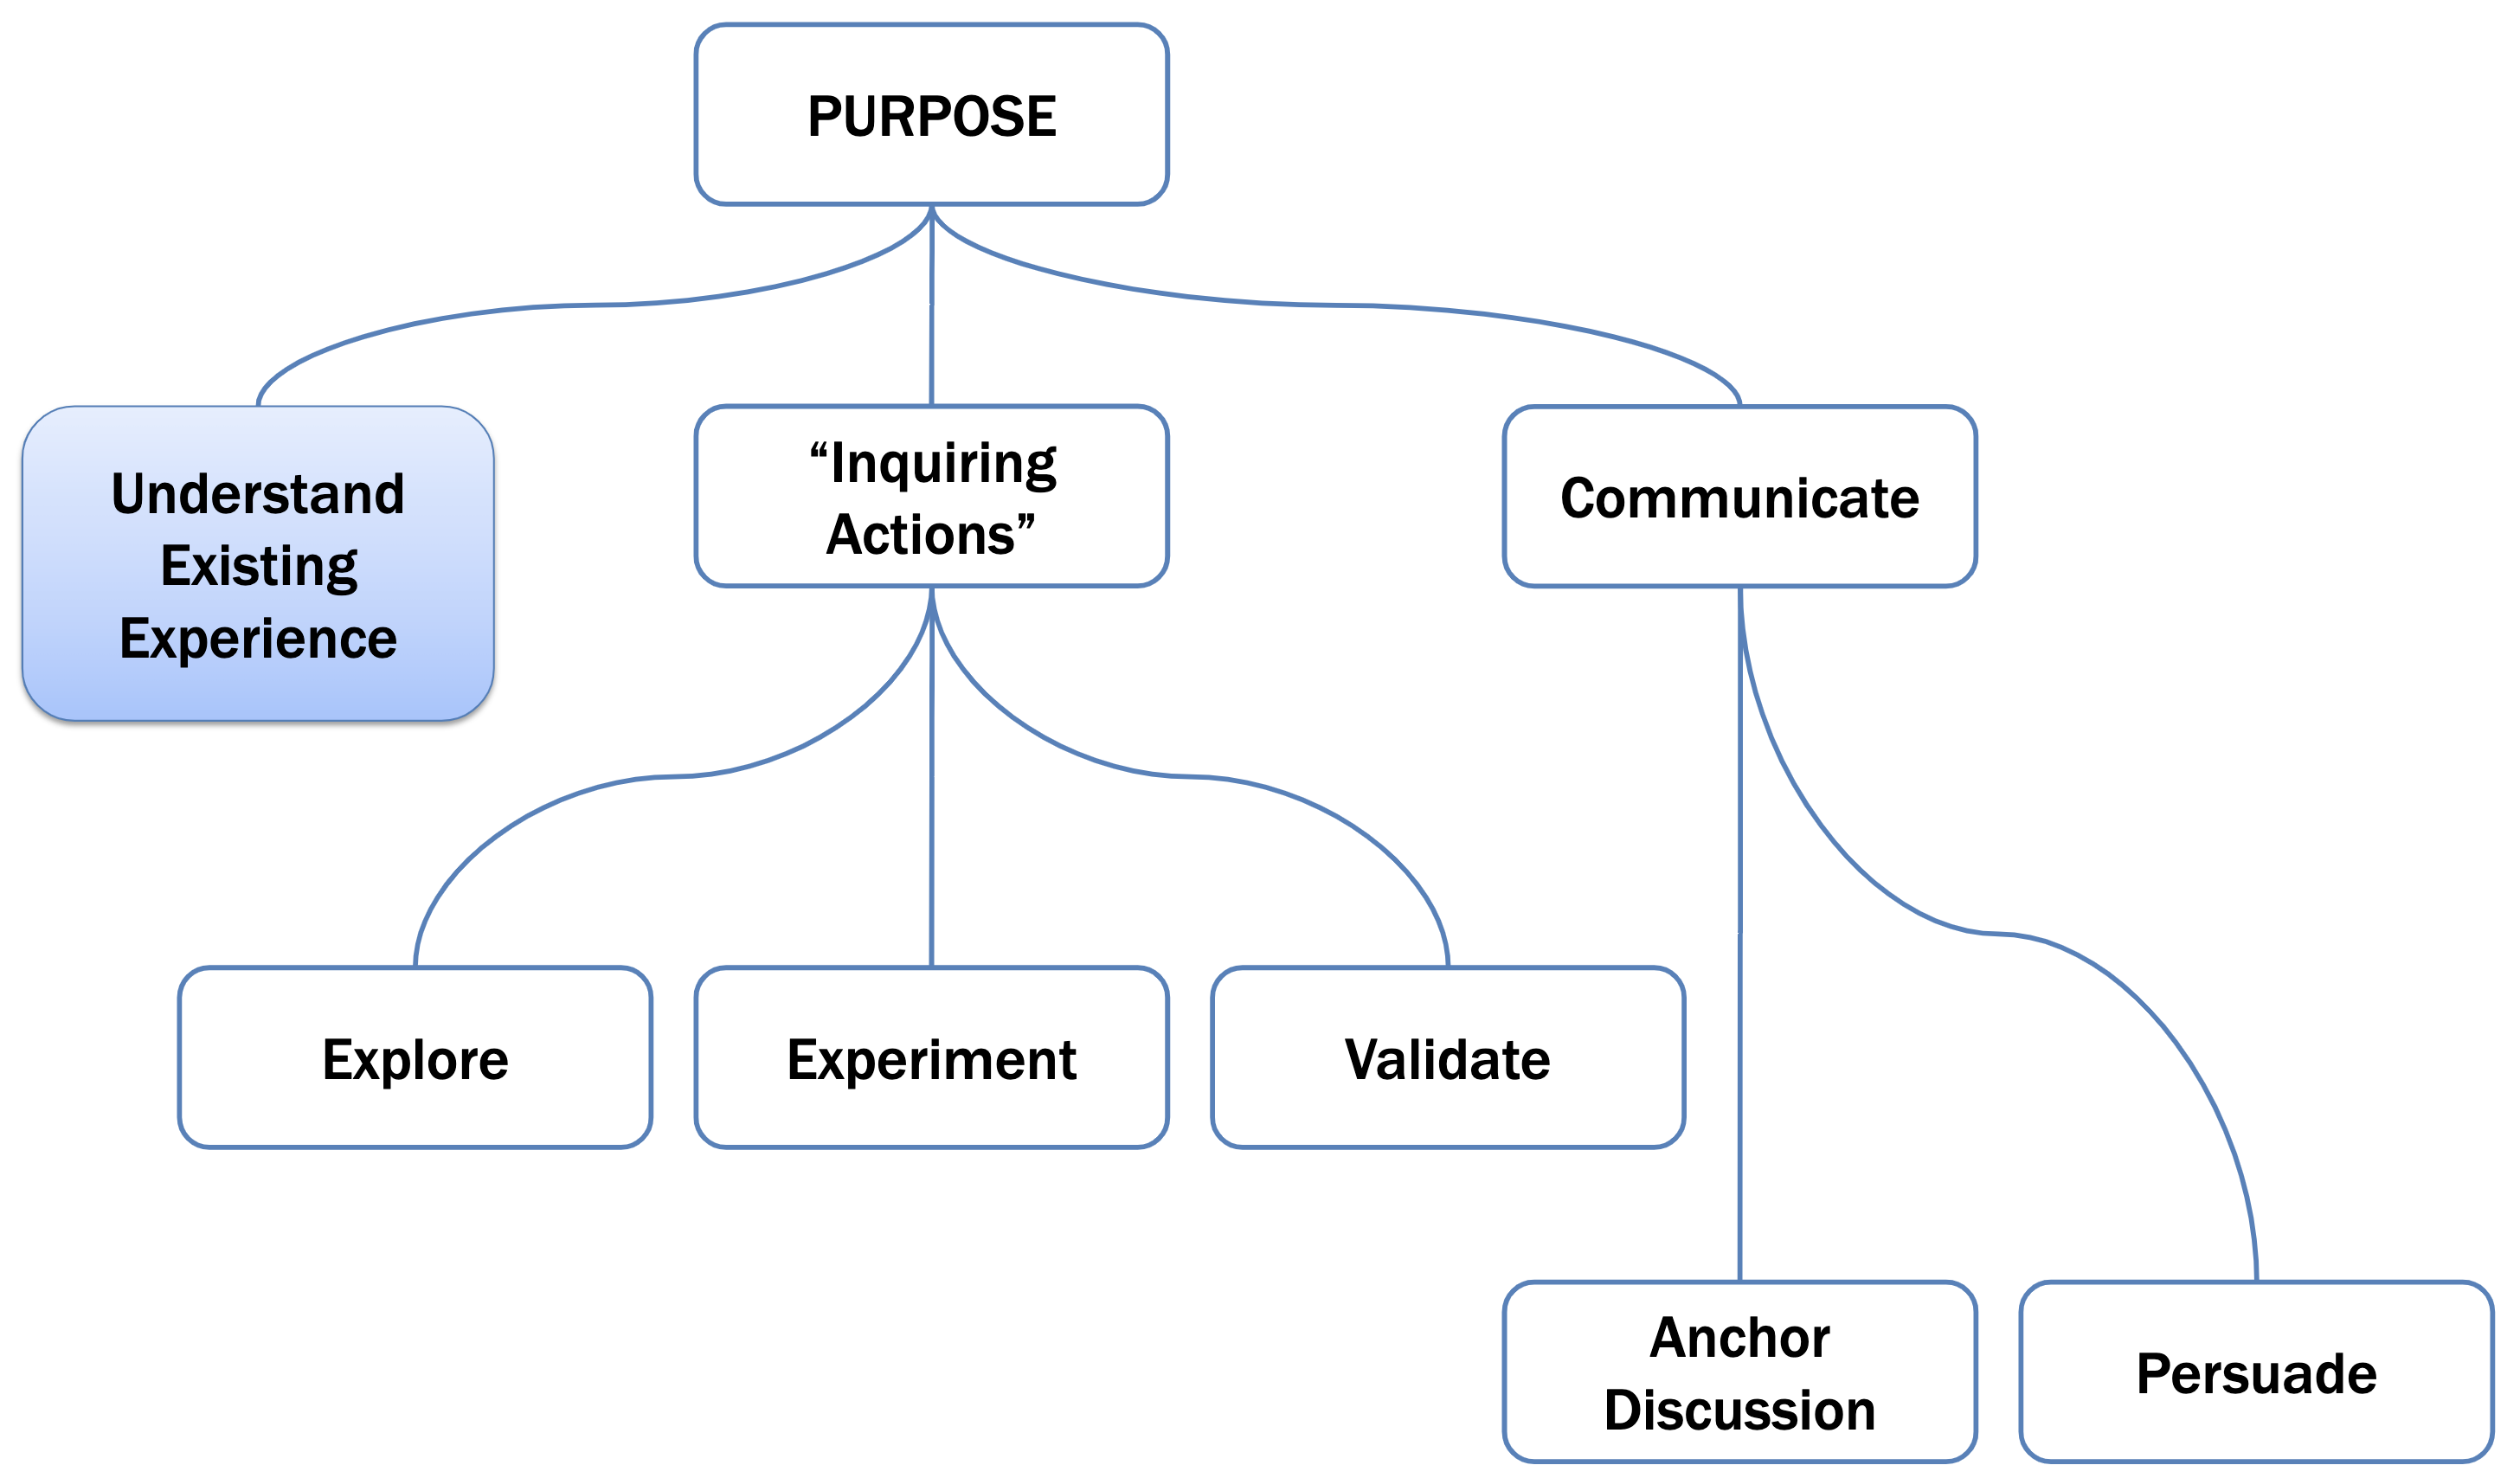
\includegraphics[scale=0.15]{lectures/wk5/img/why_prototype.png}\\
Microsoft had at least 5 different hardware prototypes of the Microsoft mouse, as well as hundreds of paper prototypes before a first version was officially released.

\subsection{Paper Prototyping}
It's hard to sink a lot of time into paper prototypes, so you won't get super attached to them (they are low fidelity).

Furthermore is is cheap and fast.

\subsubsection{Wizard of Oz Testing}
Have people test out your prototypes without letting them know what it is, allows you to get real feedback.

\subsection{Testing Device-Based Interfaces}
When conducting a test, it is preferable to have 3-4 testers.
\begin{itemize}
    \item \textbf{Greeter} - Puts users at ease \& gets data
    \item \textbf{Facilitator} - only team member who speaks
    \begin{itemize}
        \item Gives instructions \& encourages thoughts, opinions
    \end{itemize}
    \item \textbf{Computer} - knows application logic \& controls it
    \begin{itemize}
        \item Always simulates the response, w/o explanation
    \end{itemize}
    \item \textbf{Observer(s)} - Take notes \& recommendations
\end{itemize}
A typical session should be approximately \textbf{1 hour} as you have to:
\begin{itemize}
    \item Preparation
    \item The Test
    \item Debriefing
\end{itemize}

\begin{important}
    Make sure to record \textit{critical events}.

    Critical Events may also be moments when the user
    \begin{itemize}
        \item Got stuck
        \item Suddenly understood something
        \item Said ``That's cool''
        \item Said ``Ohhh'' etc. 
    \end{itemize}
\end{important}

\subsection{Prototyping in Software}
\subsubsection{Fidelity in Prototyping}
\begin{shaded}
    Fidelity refers to \textit{the level of detail}.
\end{shaded}

\begin{itemize}
    \item High fidelity: Prototypes look like the final product
    \item Low fidelity: Artists renditions with many details  missing
\end{itemize}

Paper Prototypes are low-fidelity. 

\myparagraph{Low-fidelity ``Informal'' design tools}
Examples:
\begin{itemize}
    \item DENIM (UC Berkeley)
    \item Balsamiq Wireframes
\end{itemize}
Goal is to be as rapid and flexible as physical tools.\\
Add benefits of digital media: Undo, copy+paste, resizing, etc.

\submyparagrapht{Advantages}
\begin{itemize}
    \item Takes only a few hours -- no expensive equipment needed.
    \item Can test multiple alternatives with the saved time -- faster iteration speed
    \item Can change the design as you test
    \item Especially useful for black-boxing hard to implement features such as Speech and handwriting recognition
\end{itemize}

\submyparagrapht{Disadvantages}
\begin{itemize}
    \item Can be hard to design at the proper scale / complexity  / information density of the real UI
    \item Need to re-create the interface in the target technology
    \item May not allow real-time end-user interaction
\end{itemize}

\myparagrapht{High-fidelity visual mockups}
\begin{itemize}
    \item Keynote, Powerpoint
    \item Flinto+Sketch
    \item Figma
    \item InVision
    \item Adobe Xd
\end{itemize}

\submyparagraph{Disadvantages}
\textbf{Distorts perceptions of the tester:}
\begin{itemize}
    \item Formal representation indicates “finished” nature
    \item People comment on color, fonts, and alignment
\end{itemize}

\textbf{Discourages major changes:}
\begin{itemize}
    \item Testers don’t want to change a “finished” design
    \item Sunk-cost reasoning: Designers don’t want to lose effort put into creating hi-fi design
\end{itemize}

\myparagraph{High-fidelity, fully-interactive prototypes}
Should look and behave like the final application.\\
Takes a lot of effort to build -- too little payoff -- only use as needed?

Example tools: 
\begin{itemize}
    \item HTML+CSS+Javascript
    \item Apache Cordova etc
\end{itemize}

\subsection{Video Prototyping}
Make sure to demonstrate each of the features/functionality your application will have.

Add structure to better explain content:
\begin{itemize}
    \item Begin with a title
    \item Follow with an “establishing shot”
    \item Create series of closeup \& mid-range shots, interspersed with title cards
    \item Place a final card with credits at the end
\end{itemize}

Can use stub-motion animation to help do this.
